\chapter{Resources}
\label{vl:tc-resources}


%%%%%%%%%%%%%%%%%%%%%%%%%%%%%%%%
\section{Work Breakdown Structure (WBS)}
\label{sec:fdsp-coord-wbs}

The \dword{dune} \dword{wbs} has six categories at level 1 as shown in
Table~\ref{fig:WBS_level2}.  
\begin{dunefigure}[\dword{dune} \dword{wbs} at level 2]{fig:WBS_level2}
  {High level \dword{dune} \dword{wbs} to level 2.}
  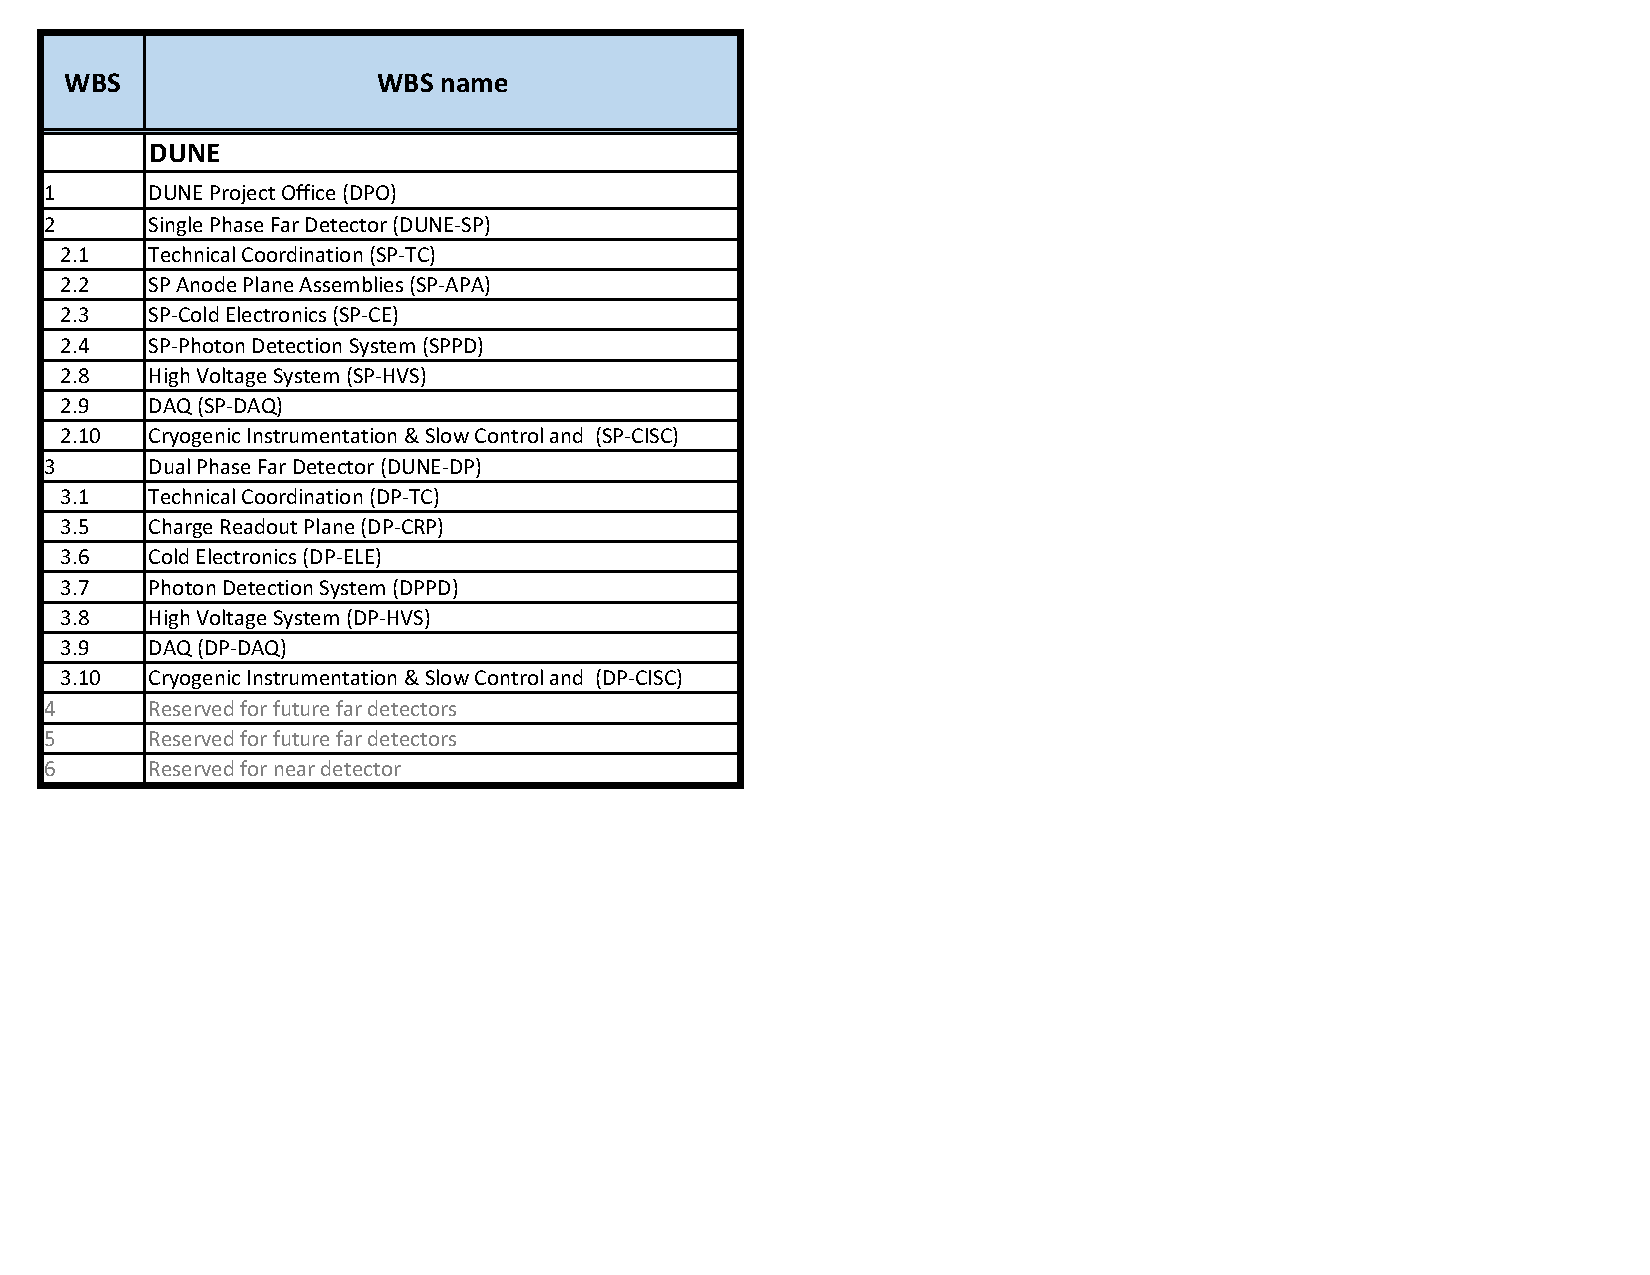
\includegraphics[width=0.75\textwidth]{WBS_level2}
\end{dunefigure}
At level 2, the \dword{wbs} breaks down into seven items, both
for single-phase and dual-phase far detectors, including the \dword{tc}
functions associated with installation.

Each subsystem \dword{wbs} is owned by the associated consortium. The
consortia \dword{wbs} follow a common format with the first level
(level 3) broken down in rough time sequence into the following
categories:
\begin{enumerate}
  \item Management
  \item Physics and Simulation
  \item Design, Engineering and R\&D
  \item Production Setup
  \item Production
  \item Integration (ITF)
  \item Installation (\surf)
\end{enumerate}
Subsequent levels in the \dword{wbs} generally follow consortia subsystem structure.
This \dword{wbs} has been used as the framework to capture the costs
for the overall \dword{dune} project cost estimate.

%%%%%%%%%%%%%%%%%%%%%%%%%%%%%%%%
\section{Cost}
\label{sec:fdsp-coord-cost}

\fixme{new standard cost table will be coming in early April - for autogenerating latex. Anne}

A preliminary \dword{dune} project cost estimate scaled from
\dword{protodune} costs was provided to the \dword{ncg} in August
2018. Based on feedback from that review and updated cost estimates
based on refined \dword{dune} designs, an updated cost estimate has
been developed and provided separately to the \dword{ncg}. A
corresponding project schedule has been developed and is discussed in
Section~\ref{sec:fdsp-coord-controls}. Cost estimates are provided for
both single-phase (\dword{dsp}) and dual-phase (\dword{ddp})
detectors. The sequencing plan is described in
Volume~\volnumberexec:~\voltitleexec. A cost summary is provided in
Table~\ref{tab:cost_L1}.
\begin{dunetable}
  [\dword{dune} Project Cost at \dword{wbs} level 1]
  {|p{0.07\linewidth}|p{0.15\linewidth}|p{0.2\linewidth}|p{0.2\linewidth}|p{0.2\linewidth}|}
  {tab:cost_L1}
  {\dword{dune} Project Cost for each detector}.
  \dword{wbs} & Detector type & Detector \#1 & Detector \#2 & Detector \#3   \\ \toprowrule
  2.0 & \dword{dsp} & &  & \\ \colhline
  3.0 & \dword{ddp} & & & \\ \colhline
\end{dunetable}

The cost estimate includes the materials and services (M\&S) cost in
local currencies in 2018, converted to 2018 US\$. The cost estimate
includes the number of labor hours broken down into eight categories
(engineer, designer, technician, student, postdoc, graduate student,
scientist, faculty). There is no escalation included in the cost estimate.
This estimate follows standard international definitions of core costs (as used
by the LHC at CERN. No design labor is included (only post-CD3 costs).

The cost estimate is for one single-phase and one dual-phase far
detector, where the sequencing assumes that a single-phase detector
comes first. This implies that some common costs are captured in the
single-phase cost estimate. The cost estimate at \dword{wbs} level two is
shown in Table~\ref{tab:cost_L2}.
\begin{dunetable}
  [\dword{dune} Project Cost at \dword{wbs} level 2]
  {|p{0.05\linewidth}|p{0.3\linewidth}|p{0.25\linewidth}|p{0.35\linewidth}|}
  {tab:cost_L2}
  {\dword{dune} Project Cost at \dword{wbs} level 2}
  \dword{wbs} & Item & M\&S & Labor hours   \\ \toprowrule
  {\bf 2.0} & {\bf \dword{dsp}} & &             \\ \colhline
  2.1 & Technical Coordination & &  \\ \colhline
  2.2 & APA & &  \\ \colhline
  2.3 & CE & &  \\ \colhline
  2.4 & PDS & &  \\ \colhline
  2.8 & HV & &  \\ \colhline
  2.9 & DAQ & &  \\ \colhline
  2.10 & CISC & &  \\ \colhline
  {\bf 3.0} & {\bf \dword{ddp}} & &             \\ \colhline
  3.1 & Technical Coordination & &  \\ \colhline
  3.5 & CRP & &  \\ \colhline
  3.6 & CE & &  \\ \colhline
  3.7 & PDS & &  \\ \colhline
  3.8 & HV & &  \\ \colhline
  3.9 & DAQ & &  \\ \colhline
  3.10 & CISC & &  \\ \colhline
\end{dunetable}


No operations costs are included. While some parts of the detector are
accessible and equipment can be maintained, other parts are not. For
those systems with accessible equipment some costs are included for
replacement over the life of the detector.

Detailed cost estimates for each subsystem are available in
\dword{dune} \dword{tdr} Volume~\volnumbersp\: \dword{dsp} and
Volume~\volnumberdp\: \dword{ddp} for each consortium. A companion
cost book for \dword{dune} contains further details.

%%%%%%%%%%%%%%%%%%%%%%%%%%%%%%%%
\section{MOU}
\label{sec:fdsp-coord-mou}

A \dword{mou} will be executed in which all deliverables will be
documented. The \dword{mou} will include the responsibilities of each
collaborating institution, their funding agency and the Host Lab for 
construction of the experiment.

%%%%%%%%%%%%%%%%%%%%%%%%%%%%%%%%
\section{Budget}
\label{sec:fdsp-coord-budget}

\dword{dune} \dword{tc} will be supported by the
\dword{comfund} and host country. The \dword{rcoord} will oversee
the \dword{comfund}.  The \dword{tc} budget will be reviewed and
approved annually by the \dword{rrb}.

%%%%%%%%%%%%%%%%%%%%%%%%%%%%%%%%
\section{Financial Change Control}
\label{sec:fdsp-coord-financialchange}

